\resizebox {\columnwidth} {!} {
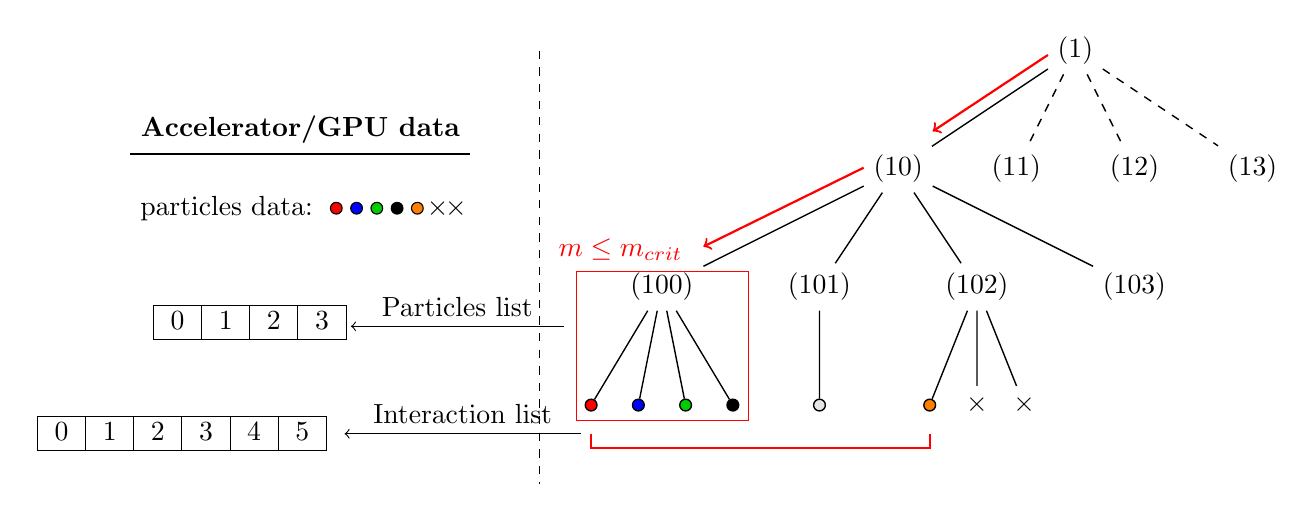
\begin{tikzpicture}

\def\da{2cm}
\def\db{20mm}
\def\dc{6mm}

\node [fill=white] at (9,0) (root) {(1)}
    child [line width=.5pt] { [sibling distance=\db] node [fill=white] (n10) {(10)}
      child {node (n100) {(100)} [sibling distance=\dc]
      	child { node[fill=red,circle,inner sep=1.5pt,draw] (n1000) {} }
      	child { node[fill=blue,circle,inner sep=1.5pt,draw] (n1001) {} }
      	child { node[fill=black!20!green,circle,inner sep=1.5pt,draw] (n1002) {} }
      	child { node[fill=black,circle,inner sep=1.5pt,draw] (n1003) {} }
      }
      child {node {(101)} [sibling distance=\dc]
      	child { node[fill=black!10,circle,inner sep=1.5pt,draw] (n1010) {} }
      }
      child {node {(102)} [sibling distance=\dc]
      	child { node[fill=orange,circle,inner sep=1.5pt,draw] (n1020) {} }
      	child { node[] (n1021) {$\times$} }
      	child { node[] (n1022) {$\times$} }
      }
      child {node {(103)} [sibling distance=\dc]
      }
    }
    child [line width=.5pt,dashed] { node [fill=white] {(11)}
    }
    child [line width=.5pt,dashed] { node [fill=white] {(12)}
    }
    child [line width=.5pt,dashed] { node [fill=white] {(13)}
    }
;
\draw[red,->,thick] ([yshift=7pt]root.south west) -- ([yshift=5pt]n10.north east);
\draw[red,->,thick] ([yshift=9pt]n10.south west) -- ([yshift=6pt]n100.north east);
\draw[red] ([xshift=-16pt,yshift=-3pt]n100.north west) rectangle ([xshift=4pt,yshift=-4pt]n1003.south east) node[anchor=west] (leaf) {};
\node[red] at ([yshift=5pt]n100.north west) {$m \leq m_{crit}$};

\draw[red,thick] ([yshift=-8pt]n1000.south) node (list_inter) {} |- ([yshift=-13pt]n1000.south) -- ([yshift=-13pt]n1020.south) -| ([yshift=-8pt]n1020.south);

% GPU Computation
\node[anchor=west,thick,font=\bf] at (-3,-1) (accel) {Accelerator/GPU data};
\draw[thick] (accel.south west) -- (accel.south east);

\node[anchor=west] at (-3,-2) (pd) {particles data:};
\node[fill=red,circle,inner sep=1.5pt,draw] at ([xshift=5pt]pd.east) (a) {};
\node[fill=blue,circle,inner sep=1.5pt,draw] at ([xshift=5pt]a.east) (b) {};
\node[fill=black!20!green,circle,inner sep=1.5pt,draw] at ([xshift=5pt]b.east) (c) {};
\node[fill=black,circle,inner sep=1.5pt,draw] at ([xshift=5pt]c.east) (d) {};
\node[fill=orange,circle,inner sep=1.5pt,draw] at ([xshift=5pt]d.east) (e) {};
\node[inner sep=1.5pt] at ([xshift=5pt]e.east) (f) {$\times$};
\node[inner sep=1.5pt] at ([xshift=1pt]f.east) (g) {$\times$};

\draw[->] (2.5,-3.5) -- ([xshift=-2.7cm]2.5,-3.5) node[midway,above] (leaf_node) {Particles list};
\node[anchor=east] at ([xshift=-.2cm,yshift=-.2cm]leaf_node.west) { 
	\begin{tabular}{|c|c|c|c|}
		\hline
		0 & 1 & 2& 3\\
		\hline
  	\end{tabular}	
};
\draw[->] (list_inter.west) -- ([xshift=-3cm]list_inter.west) node[midway,above] (inter) {Interaction list};
\node[anchor=east] at ([xshift=-3.1cm]list_inter.west) { 
	\begin{tabular}{|c|c|c|c|c|c|}
		\hline
		0 & 1 & 2 & 3 & 4 & 5\\
		\hline
  	\end{tabular}	
};

\draw[dashed] (2.2,0) -- (2.2,-5.5);


\end{tikzpicture}
}